Pour réaliser ce projet, nous avons choisi de faire de l'Agile, avec la méthode SCRUM. Faire de l'Agile permet d'avoir un rendu fonctionnel à chaque fin de sprint, et donc de s'assurer d'avoir un rendu final. De plus, c'est une manière de faire qui se dévellope en entreprise, nous voulions donc l'expérimenter.
\section{Backlog}
Nous avons commencer le projet avec un sprint 0, au cours duquel nous avons défini l'univers du projet, et ses fonctionnalités (backlog).\\

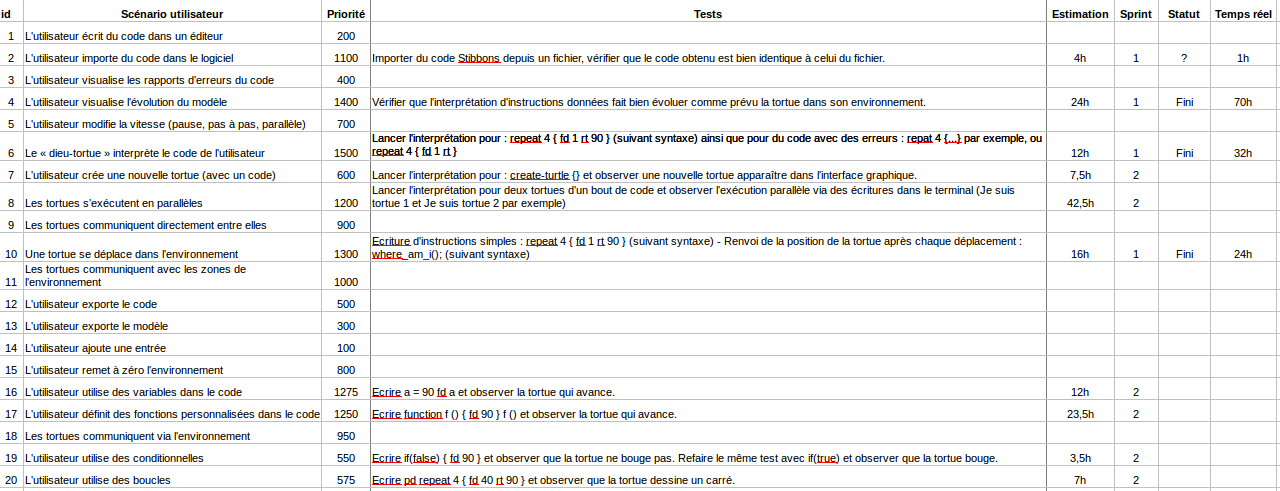
\includegraphics[scale=0.3]{doc/report/uml/backlogv1.png}
Le backlog est composé de fonctionnalités, qui ont un indice entre 1000 et 0 pour leur importance du rendu final. On écrit aussi une "user-storie" pour chaque fonctionnalité. Cela correspond au test que l'on fait passer au programme pour valider la fonctionnalité.
A chaque sprint, on décide des fonctionnalités qu'on ajoute, et du nombre d'heures qu'on estime devoir y passer.\\
